\subsection{(Speculative) Extension to non-linear/uncertain agents} 
%%%%%%%%%%%%%%%%%%%%%%%%%%%%%%%%%%%%%%%%%%%%%%%%%%%%%%%%%%%%%%%%%%%%%
%%%%%%%%%%%%%%%%%%%%%%%%%%%%%%%%%%%%%%%%%%%%%%%%%%%%%%%%%%%%%%%%%%%%%
\subsubsection{Double integrator agents to general non-linear agents}
\begin{frame}{Double integrator agents to general non-linear agents}
	\begin{figure}[h!]
		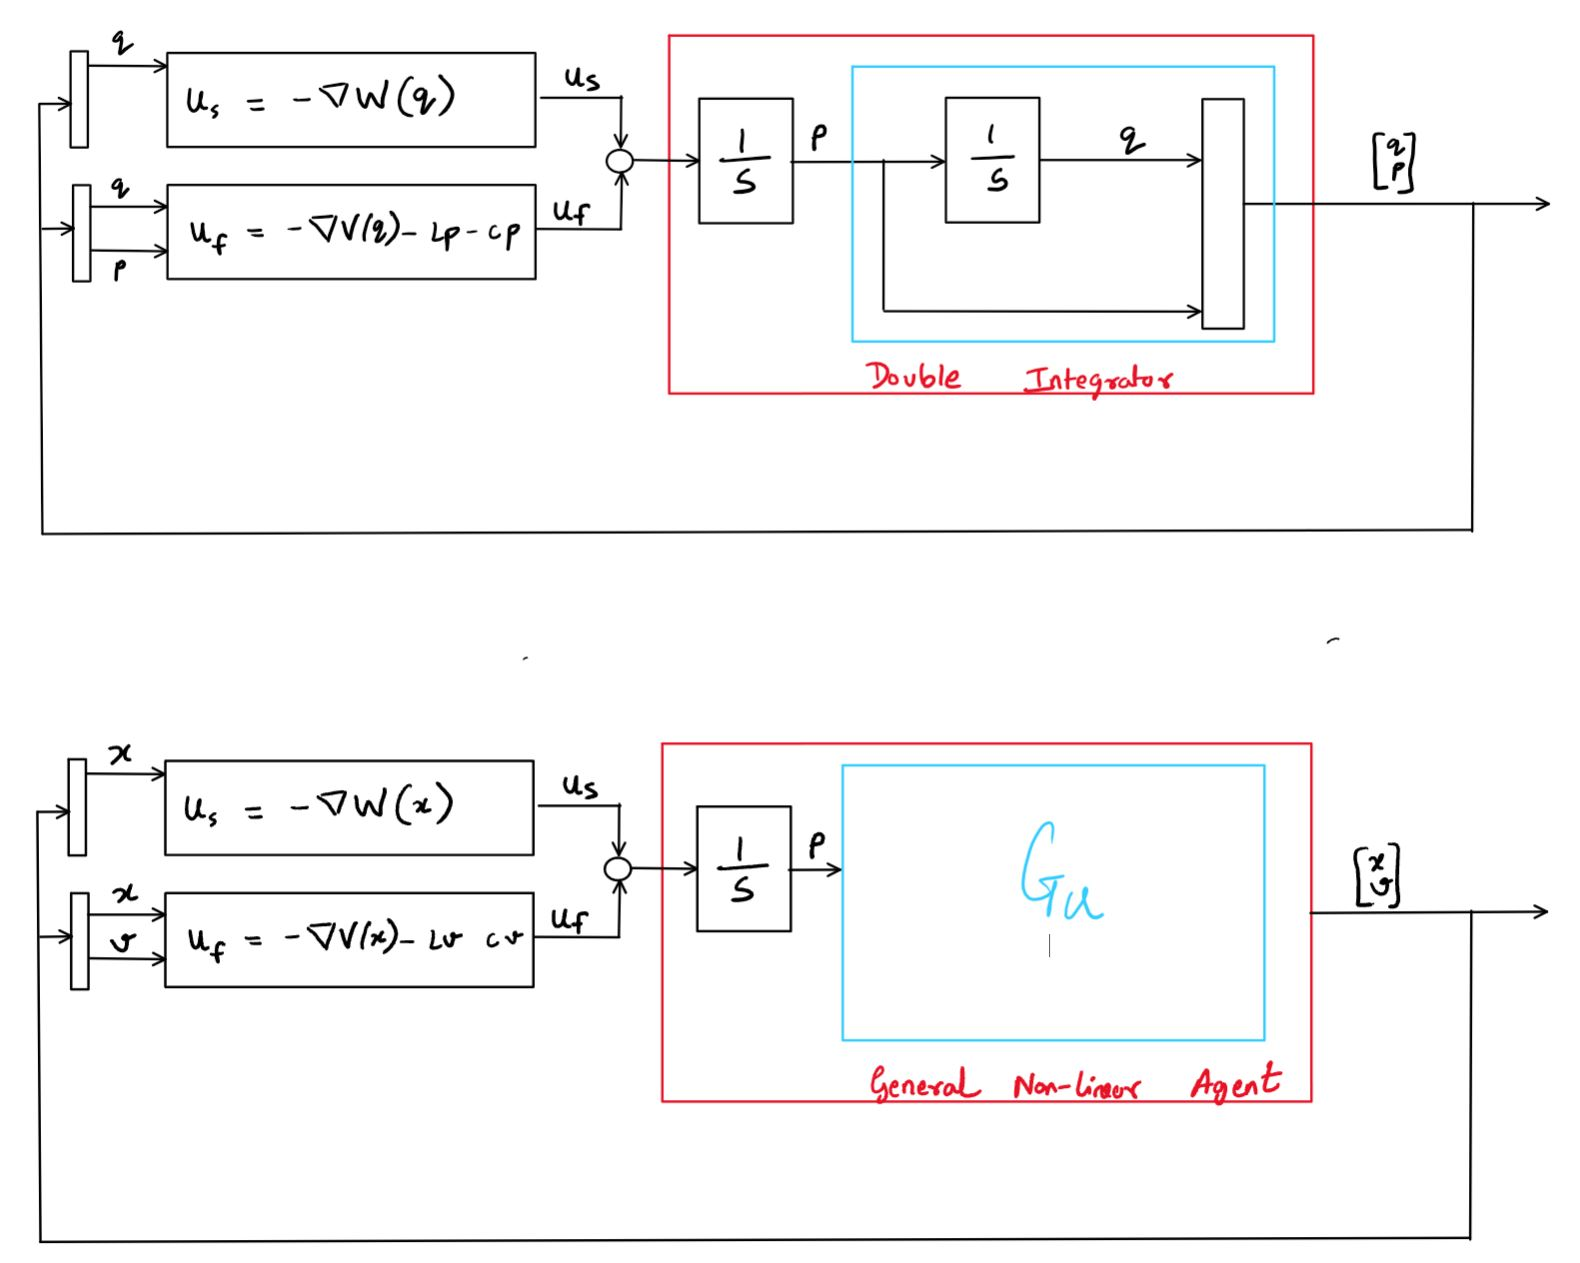
\includegraphics[width=10cm]{doc/1_Flocking_source_seek/double_integrator_to_general_agents_slide.jpg}
		%\caption{}
		\label{fig:control_arch}	
	\end{figure}	
\end{frame}
%%%%%%%%%%%%%%%%%%%%%%%%%%%%%%%%%%%%%%%%%%%%%%%%%%%%%%%%%%%%%%%%%%%%%
\begin{frame}{Double integrator agents to general non-linear agents}
Dynamics with double integrator:
\begin{equation*}
\begin{split}
\Dot{q}&=p\\
\Dot{p}&=-\nabla V(q)-\hat{L}(q)p -cp\textcolor{red}{-k_1\nabla^2 \Psi(q) p -k_2 \nabla \Psi(q)}
\end{split}
\end{equation*}	
Dynamics with general agents:
\begin{equation*}
\begin{split}
\begin{bmatrix}
x\\v
\end{bmatrix}&=G_{\textnormal{cl}}p\\
\Dot{q}&=p\\
\Dot{p}&=-\nabla V(\textcolor{blue}{x})-\hat{L}(\textcolor{blue}{x})\textcolor{blue}{v} -c\textcolor{blue}{v}\textcolor{red}{-k_1\nabla^2 \Psi(\textcolor{blue}{x}) \textcolor{blue}{v} -k_2 \nabla \Psi(\textcolor{blue}{x})}
\end{split}
\end{equation*}			
\end{frame}
%%%%%%%%%%%%%%%%%%%%%%%%%%%%%%%%%%%%%%%%%%%%%%%%%%%%%%%%%%%%%%%%%%%%%
\begin{frame}{Double integrator agents to general non-linear agents}
\textbf{Core Idea:}
\\
Under  
\begin{itemize}
\item a Lipschitz condition on the underlying scalar field 
\item a Lipschitz condition on the interaction field
\item $L_2$ bound on the tracking error of the local closed loop, $G_{\textnormal{cl}}$
\end{itemize}
the dynamics for general agents could be written as:
\begin{equation*}
\begin{split}
\Dot{q}&=p\\
\Dot{p}&=-\nabla V(q)-\hat{L}(q)p -cp\textcolor{red}{-k_1\nabla^2 \Psi(q) p -k_2 \nabla \Psi(q)} + \textcolor{blue}{d}\\
||d_T||&\leq K ||p_T||_{L_2} \forall T
\end{split}
\end{equation*}	
\begin{itemize}
\item Standard dissipativity based arguments to show stability (Boundedness of trajectories)
\item Assymptotic stability not shown !
\end{itemize}
\end{frame}
%%%%%%%%%%%%%%%%%%%%%%%%%%%%%%%%%%%%%%%%%%%%%%%%%%%%%%%%%%%%%%%%%%%%%
\begin{frame}{Double integrator agents to general non-linear agents}
A speculative idea
\begin{itemize}
	\item IQCs can be used efficiently to get upper bounds on robust exponential decay rates\footnote{Boczar, R., Lessard, L., Packard, A. and Recht, B., 2017. Exponential stability analysis via integral quadratic constraints. arXiv preprint arXiv:1706.01337.}
	\item Can be possibly applied to LPV systems to obtain exponential decay rates under parameter variation
	\item These rates could be then used with a singular perturbation and a regular perturbation argument to prove asymptotic stability of the overall system
	\item The linear analogue would be to consider the slowest eigen values of the closed loop agent dynamics
\end{itemize}
\end{frame}
%%%%%%%%%%%%%%%%%%%%%%%%%%%%%%%%%%%%%%%%%%%%%%%%%%%%%%%%%%%%%%%%%%%%%
\begin{frame}{Other speculative ideas we have in mind}
	\
	\begin{itemize}
		\item Adapt the flocking algorithm coefficients online based on the measured error such the $\dot{E}<0$. (Borrowing ideas from adaptive control)
		\item Similar to ideas in \footnote{Chopra, N. and Spong, M.W., 2006. Passivity-based control of multi-agent systems. In Advances in robot control (pp. 107-134). Springer, Berlin, Heidelberg.}, design local tracking control for passivity and use the fact the interconnections of passive systems is passive.
	\end{itemize}
\end{frame}
%%%%%%%%%%%%%%%%%%%%%%%%%%%%%%%%%%%%%%%%%%%%%%%%%%%%%%%%%%%%%%%%%%%%%